\documentclass[10pt]{beamer}
\usepackage[utf8]{inputenc}
\usepackage[russian]{babel}

\newcommand{\pder}[2] {\frac{\partial #1}{\partial #2}}
\newcommand{\ppder}[2]{\frac{\partial^2 #1}{\partial {#2}^2}}
\newcommand{\pcder}[3]{\frac{\partial^2 #1}{\partial #2 \partial #3}}
\newcommand{\der}[2]  {\frac{d #1}{d #2}}
\newcommand{\dder}[2] {\frac{d^2 #1}{d {#2}^2}}

\newcommand{\const}{\mathrm{const}}                     
\newcommand{\average}[1]{\left\langle #1 \right\rangle} 
\newcommand{\abs}[1]{\left| #1 \right|}                 
\newcommand{\ds}{\displaystyle}                         
\newcommand{\D}{\Delta}
\newcommand{\dotunder}[1]{\d{#1}} 
\renewcommand{\d}{\delta}
\newcommand{\eps}{\varepsilon}
\renewcommand{\phi}{\varphi}

\newcommand{\divergence}{\mathrm{div\,}}  
\newcommand{\gradient}  {\mathrm{grad\,}} 
\newcommand{\rotor}     {\mathrm{rot\,}}  

\usetheme{Hannover}
\date{Волгоград, 2014}
\title{Модификация уравнения Нернста--Планка для пассивного транспорта}
\author{Абдрахманов В. Л.}
\begin{document}
  \frame{\titlepage}
  \begin{frame}
    \frametitle{Введение}

    \textbf{Актуальность.} Экспериментально установлено, что наличие
    высокочастотных полей влияет на процессы движения ионов, причем это
    влияние в большой степени зависит от уровня падающей мощности.
    Наличие высокочастотных полей в настоящее время является постоянным
    фактором, поэтому изучение его влияния на живой организм необходимо.
    Таким образом, создание моделей, позволяющих описать этот процесс
    хотя бы с учетом ограничений и приближений, является актуальной
    задачей.

    \textbf{Цель работы} заключается в получении уравнений, описывающих
влияние высокочастотных возмущений на ионные токи в мембранах. При
рассмотрении задачи ионного транспорта в электродиффузионном подходе
используется уравнение Нернста—Планка, которое применимо в
стационарном случае, то есть когда ток постоянен. Так как электрические
колебания не стационарный процесс, то необходимо модифицировать
уравнение для нестационарного случая.
\end{frame}
  \begin{frame}
    \frametitle{Уравнение Нернста--Планка}
    \[
        j_k = -\frac{z_k}{\abs{z_k}}u_kRT\pder{c_k}{x} -
        \abs{z_k}u_kc_kF\pder{\phi}{x}.
        \label{eq:nernst-plank}
    \]

      \textbf{Приближённое решение Планка}
      \[
          c(x) = \chi x + c(0),\ \chi = \frac{c(\delta)-c(0)}{\delta},
      \]
      \[
          \phi = \frac{\alpha}{\chi}\ln\frac{\chi\delta + c(0)}{c(0)},
          \ \alpha = \frac{\phi[c(\delta) - c(0)]}
          {\delta\ln[c(\delta) / c(0)]}.
      \]
      \textbf{Приближённое решение Гольдмана}
      \[
          \phi(x) = \phi(0) - Ex,
      \]
      \[
          c_k(x) = c_k(0) + [c_k(\delta) - c_k(0)]
          \frac{e^{z_k\beta Ex} - 1}{e^{z_k\beta E\delta} - 1}.
      \]
  \end{frame}
  \begin{frame}
      \frametitle{Нестационарное уравнение}
        \[
          j = -\frac{z}{|z|}ukT\pder{n}{x} - |z|nue\pder{\phi}{x}.
        \]
        \[
            \pder{\rho}{t} + \divergence\vec{j} = 0.
        \]
        Учитывая, что \( \rho = nez \), получим уравнение
        \[
            \pder{n}{t} = \frac{ukT}{e|z|}\ppder{n}{x} +
            \frac{z}{|z|}u\pder{\phi}{x}\pder{n}{x} +
            \frac{z}{|z|}u\ppder{\phi}{x}n.
        \]
  \end{frame}
  \begin{frame}
      \frametitle{Решение для планковского и гольдмановского приближений}
      \textbf{Планковское приближение}

      \begin{minipage}{.3\textwidth}
          \begingroup
\everymath{\scriptstyle}
\scriptsize
        \begin{align*}
        & \pder{n}{\tau} = \ppder{n}{\xi} - wg(\xi)\pder{n}{\xi} + wg^2(\xi)n,
            \ \xi\in(0,1) \\
        & \tau = \frac{D}{d^2}t,\ \xi = \frac{x}{d},\ w = \frac{vd}{D},
        \ g(\xi) = \frac{1}{\xi - \frac{n_{out}}{n_{out} - n_{in}}},\\
        & n(0, \tau) = n_{out},\ \tau>0 \\
        & n(1, \tau) = n_{in},\ \tau>0 \\
        & n(\xi, 0) = 0,\ \xi\in(0,1).
    \end{align*}
\endgroup
\end{minipage}\hfill
      \begin{minipage}{.3\textwidth}
    \begin{figure}[H]
    \begin{center}
        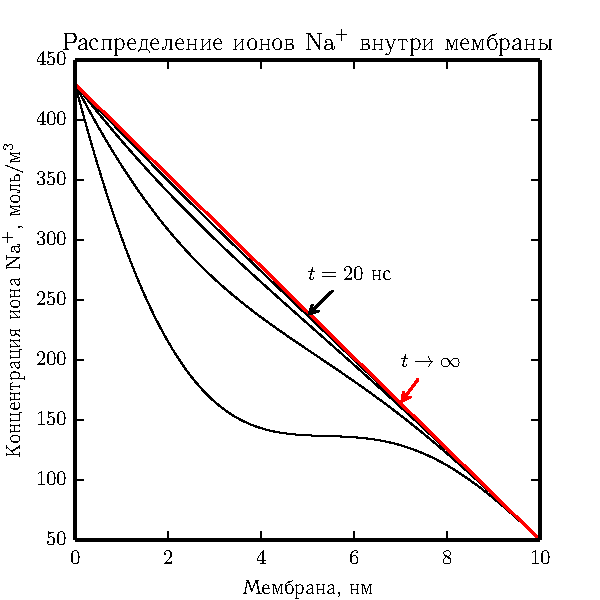
\includegraphics[width=\textwidth]{../plots/linear_conc}
    \end{center}
    \end{figure}
\end{minipage}


      \textbf{Гольдмановское приближение}

      \begin{minipage}{.47\textwidth}
\begingroup
\everymath{\scriptstyle}
\scriptsize
        \begin{align*}
            & \pder{n}{\tau} = \ppder{n}{\xi} -
                w\pder{n}{\xi},\ \xi\in(0,1) \\
            & \tau = \frac{D}{d^2}t,\ \xi = \frac{x}{d},\ w = \frac{vd}{D},\\
            & n(0, \tau) = n_{out},\ \tau>0 \\
            & n(1, \tau) = n_{in},\ \tau>0 \\
            & n(\xi, 0) = 0,\ \xi\in(0,1).
        \end{align*}
\endgroup
    \end{minipage}\hfill
      \begin{minipage}{.3\textwidth}
     \begin{figure}[H]
    \begin{center}
        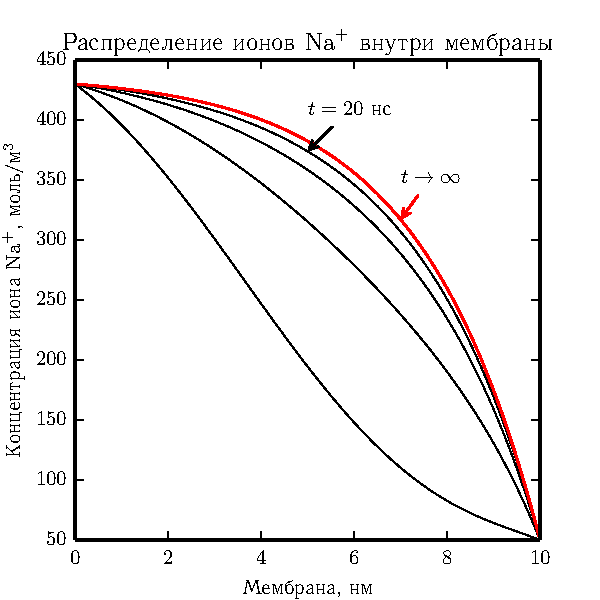
\includegraphics[width=\textwidth]{../plots/linear_field}
    \end{center}
    \end{figure}
\end{minipage}


  \end{frame}
  \begin{frame}
      \frametitle{Учёт уравнения Пуассона}
      \[
          E = E_{ex} + E_{in}.
      \]
      \[
        \pder{E_{in}}{x} = \frac{cFz}{\eps\eps_0},\quad
        c = \frac{\eps\eps_0}{Fz}\pder{E_{in}}{x}.
    \]
    \[
        j = \eps\eps_0
            \left(-D_i\ppder{E_{in}}{x}+\frac{z_i}{|z_i|}u_iE\pder{E_{in}}{x}\right).
        \label{eq:j_from_E}
    \]
    \[
        \pder{\rho}{t} + \pder{j}{x} = 0.
    \]
    \[
        \pder{j}{x} = -\eps\eps_0\pcder{E_{in}}{x}{t}.
        \label{eq:displacement-current}
    \]
    \[
        \pcder{E}{x}{t} = D\frac{\partial^3{E}}{\partial x^3} -
        \frac{z}{\abs{z}}\frac{u}{2}\ppder{E^2}{x}.
        \label{eq:epic-equation}
    \]
    Граничное условие
    \[
        \left.\pder{E}{x}\right|_{x=0} = \frac{Fz}{\eps\eps_0}c(0),\quad
        \left.\pder{E}{x}\right|_{x=d} = \frac{Fz}{\eps\eps_0}c(d).
    \]
    \end{frame}
  \begin{frame}
    \frametitle{Добавление СВЧ-поля}
    \[
        E = E_m e^{i\omega t} + E^{(0)} + E^{(1)} + \ldots,\ |E_m| << E^{(0)}.
    \]
    \begin{gather*}
    \pcder{E^{(1)}}{x}{t} = D\frac{\partial^3 E^{(1)}}{\partial x^3} +
    \frac{uzE^{(0)}}{\abs{z}}\ppder{E^{(1)}}{x} +
    2\frac{uz}{\abs{z}}\pder{E^{(0)}}{x}\pder{E^{(1)}}{x} +\\+
    \frac{uz}{\abs{z}}\ppder{E^{(0)}}{x} E^{(1)} +
    \frac{uz}{\abs{z}}\ppder{E^{(0)}}{x} E_m e^{i\omega t}.
\end{gather*}
  \end{frame}
  \begin{frame}
      \frametitle{Заключение}
      В данной работе предпринята попытка получить эквивалент уравнения
Нернста—Планка для нестационарного процесса. Получено уравнение, которое может быть использовано для рассмотрения нестационарного
процесса переноса ионов в мембране, однако его недостатком является то,
что для его решения требуется явный вид профиля потенциала в мембране. В
качестве попытки обойти эту проблему, было получено уравнение,
которое включает в себя только одну неизвестную функцию. Но и это
уравнение в том виде, в котором оно получено, не может решить
поставленную задачу, так как для постановки краевой задачи требуется 3
граничных условия, в то время как у нас имеется только 2. Тем не менее,
если удастся решить эту проблему, то данное уравнение можно будет
использовать для описания транспорта ионов в мембране при наличии
высокочастотного поля.
  \end{frame}
\end{document}
